%File: formatting-instruction.tex
\documentclass[letterpaper]{article}
\usepackage{aaai}
\usepackage{times}
\usepackage{helvet}
\usepackage{courier}
\usepackage{graphicx}
\usepackage{subfigure}
\usepackage[hyphens]{url}
\usepackage[numbers, sort]{natbib}
\usepackage[section]{placeins}
\frenchspacing
\setlength{\pdfpagewidth}{8.5in}
\setlength{\pdfpageheight}{11in}
\pdfinfo{
/Title (Analysis of Chord Functions in the Bach Chorales Using Hidden Markov Modeling)
/Author (Rupert Deese)}
\setcounter{secnumdepth}{0}  
 \begin{document}
% The file aaai.sty is the style file for AAAI Press 
% proceedings, working notes, and technical reports.
%
\title{Analysis of Chord Functions in the Bach Chorales Using Hidden Markov Modeling}
\author{Rupert Deese\\
CS 151: Artificial Intelligence\\
Harvey Mudd and Pomona Colleges Joint Computer Science Department\\
}
\maketitle
\begin{abstract}
\begin{quote}
We attempt to replicate a technique described in a forthcoming paper that deduces musical grammar from a collection of musical works by training a hidden Markov models on them. K-means clustering is used to consolidate the results of many randomly initialized HMMs into a single characteristic model. We verify that a 3-state model gives a grammar that best fits the Bach chorales. Due to inconsistent results from the HMM training and decoding, the relative performance of models with more than three states is ambiguous. The chord functions and transitions of the 3-state model reflect basic notions of musical structure, most notably the pre-dominant, dominant, tonic cycle.
\end{quote}
\end{abstract}

\section{Introduction}
Most music contains more than one melodic voice. Multiple voices in harmony create a chord, one of the basic functional units of Western music and musical analysis. Although, as the composer Max Reger is said to have declared, "any chord can follow any other chord", Western music exists in relation to, and mostly follows, a set of harmonic rules \cite{harrison1994harmonic}.

These rules are aptly compared to those that govern natural language, and can be called a musical grammar. A musical grammar explains the structure of music by reducing the combination of voices in a piece of music at any given moment (voices, guitar, bass, piano, etc) to a chord. The grammar defines equivalence classes of chords called chord functions, and rules that govern the transitions between chord functions.

If we think of a musical grammar as a collection of states representing a chord functions, each with high probabilities of 'emitting' the chords characteristic of that state, and each with a high probability of transitioning to another state if there is a rule allowing a transition between the corresponding chord functions, we have a mild, but still reasonably accurate, abstraction of a musical grammar.

This paper, seizing on the correspondence between that abstraction and the hidden Markov model, presents an approach to characterize musical grammar by creating a hidden Markov model that is characteristic of a group of musical compositions. Such an approach has the potential to verify, expand upon, or complicate existing chord function theories, by inferring functional groupings based solely on chord contexts.

\section{Related Works}
This paper does not present original research. It describes an effort to replicate work done by Christopher White, and follows his methodology as closely as possible \cite{white, white2}.

\section{Background}
It is important to qualify, with respect to the introduction as well as all that follows, that the musical grammar and music theory described in this paper is most pertinent to Western classical music, and consequently also of great relavance to Western music following the Classical period. Other musics almost certainly have grammars of their own, but this paper makes no claims about those grammars.

\begin{figure}
\vspace{-100pt}
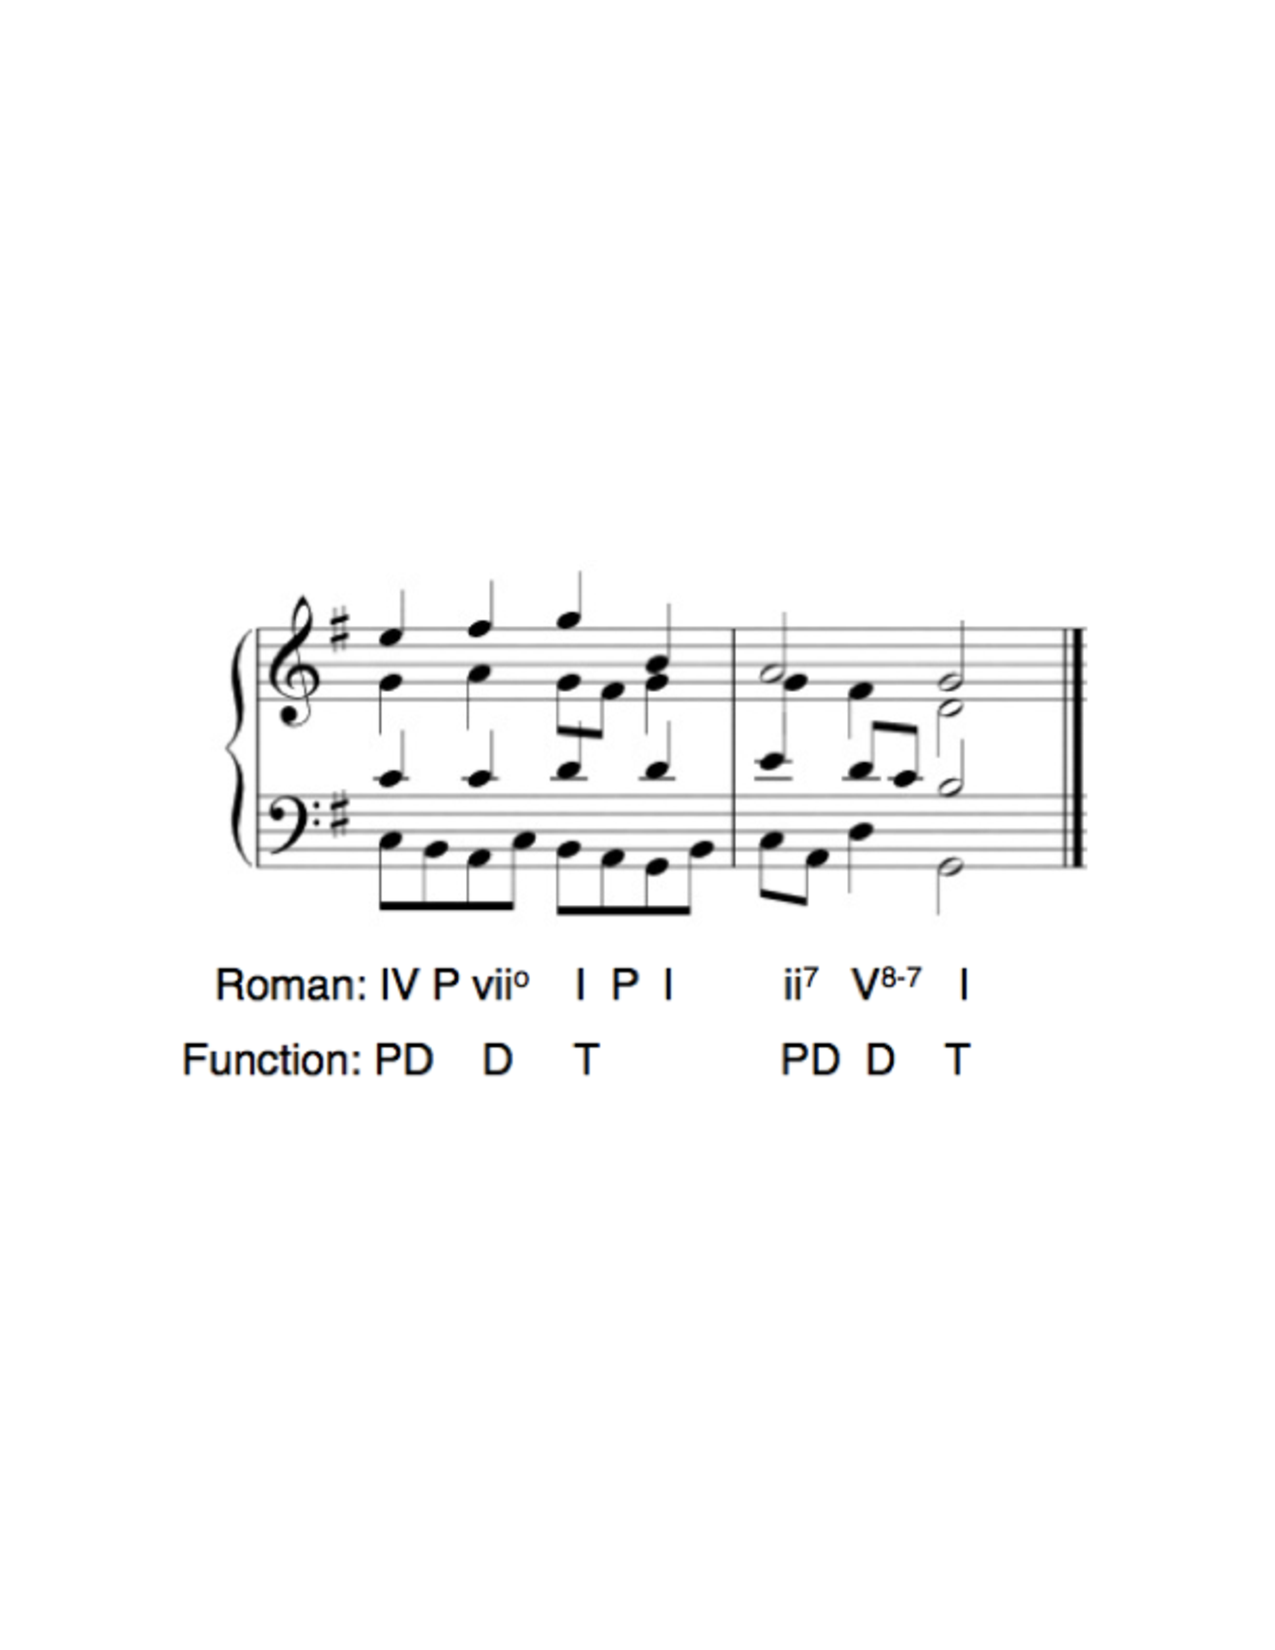
\includegraphics[width=3in]{tpd.pdf}
\vspace{-100pt}
\caption{Measures 3 and 4 of Bach's chorale \emph{Straf' mich nicht in deinem Zorn}. The first line of roman numerals is a reduction of the four voices in the chorale to chords. The line below labels the chords according to their function.}
\end{figure}

Chords are the functional units of musical grammar, analogous to words in natural language. Figure 1 shows a typical chord function analysis of a four-voice chorale written by J.S. Bach. The chords, on the first line, are labeled according to the key of the chorale, which is G major (a G chord is a I, an A minor chord is a ii, and so on). The function of each chord is then distilled from these labels. The chorale in Fig. 1 also shows adherence to the corresponding rules that dictate allowed progressions between chord functions. For example, the pre-dominant, dominant, tonic cycle, one of the most enduring structures of Western music, appears once in each measure. A musical grammar consists of chord functions and the rules that determine allowed sequences of them.

Musical grammars first received explicit attention when Noam Chomsky introduced formal grammars in the study of natural language. Chomsky's context-free grammars specify not just neighborly relations of elements in a grammar, but overall structural requirements. Musical grammars are likewise termed "generative," consisting not just of correctly adjacent chords but of phrases, forms, and movements \cite{rohrmeier2011towards}. Context-free grammars and their relatives can be very complex, but simpler grammars can still be powerfully descriptive, and are easier to produce experimentally. Claude Shannon, for example, effectively modeled English as a Markov process for the purposes of information theory \cite{shannon2001mathematical}.

A Markov model is a stochastic model in which the probability of the next state depends only on the current state; each state has its own fixed probability of transitioning to each other state. A Hidden Markov model (HMM), consists of an underlying Markov model who's states are hidden. Instead, each state has a probability of emitting each possible piece of evidence. An HMM can be trained algorithmically using a dataset, so that its transition and emission probabilities are tailored to produce the data with high likelihood. HMMs have been used successfully to process natural language \cite{saul1997aggregate}.

The dataset used in this study is the 371 chorales written by J. S. Bach. Their Baroque style is exemplary of Western classical musical grammar, and makes chord reduction easy. The statistical properties of harmony in the Bach chorales have been explored before, and grammars have been developed that produce them \cite{baroni1983concept, rohrmeier2008statistical}.

\section{System Description}
The data analysis was done in three steps: data collection, HMM modeling, and clustering. Data was collected using the \emph{music21} python package, which provides the Bach chorale corpus as a sample dataset \cite{cuthbert2010music21}. The chorales were processed one by one into a collection of sequences for use as input to the HMMs. Each chorale was reduced to chords by extracting a chord from the chorale at every moment that a voice changes in pitch. The key of each chord was determined in context using the Bellman-Budge windowing algorithm, with an 8-chord window: each chord was associated with eight key-guesses, and was accepted if all eight agreed \cite{cuthbert2010music21}. Any contiguous group of chords in the same major key was transposed into C major and used as a sequence. The sequences were then further edited by removing the 40\% least likely chords in all sequences, and by removing chords that were identical to, or a small subset of, one of their neighbors. If a least likely chord was removed from the middle of a sequence, the sequence was split into two at that location.

Discrete HMMs were implemented using the \emph{GHMM} python package \cite{ghmm}. For HMMs with 3-15 states (inclusive) 50 HMMs were tested as follows. The transition, emission, and initial state probabilities of each HMM were randomly initialized. The HMMs were trained on all bigram transitions in the sequences using the Baum-Welch algorithm, and then used to decode 20\% of the sequences, assigning a state to each chord, with the Viterbi algorithm. The state assignments were collected in a 50-element vector for each chord. A distance matrix of the chords was constructed, in which the $ij$th entry was the square of the number of differences between the $i$th and $j$th chords in the decoded sequences.

The $k$-means algorithm implemented in the \emph{scikit-learn} python package \cite{pedregosa2011scikit} was used to cluster the matrix, with $k$ equal to the number of states in the HMMs. The clustering grouped chords with similar vectors, meaning they had been assigned similarly by all 50 HMMs. Chords clustered together were considered to belong to the same state of the characteristic $k$-state HMM averaging all 50 trials.
Emission and transition probabilities, and the overall likelihood of each state, were determined by analyzing the decoded sequences and the cluster assignment of each chord. The results of clustering were evaluated by their silhouette score, or the average silhouette width over all vectors.

\section{Results}
The results are evaluated based on their agreement with the results found in White's work. Each figure references a specific figure from \emph{White, 2013} for comparison \cite{white}.

In the sequences extracted from the chorales, 209 unique chords were found (out of ${12 \choose 4} = 495$ possible combinations of the 12 semitonal pitch classes). The 84 least common of these were removed. The most common chords were I, V, $\mathrm{V^7}$, IV, vi,  $\mathrm{ii^7}$, and ii.

Figure 1 shows representative silhouette score graphs from two runs. A global maximum is observed for the $k=3$ solution. White also finds a global maximum at $k=3$, but his silhouette scores for $k > 3$ are more robust over multiple runs, while ours varied widely over different runs of the HMMs. Our silhouette scores are significantly lower than White's, and we do not find a clear local maximum at $k=13$, only that silhouette score decreases as the number of states increases.

\begin{figure}
\vspace{-10pt}
    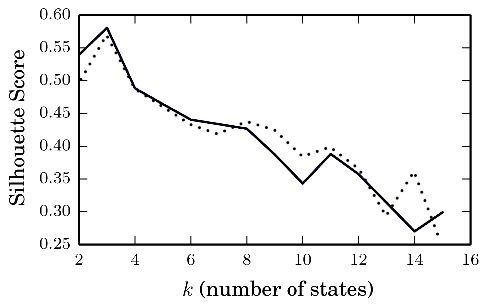
\includegraphics[width=\columnwidth]{fig1.pdf}
\label{fig:first_sub}
\vspace{-10pt}
    \caption{Silhouette width as a function of $k$ for two identical runs of 50 models each [(a) solid line; (b) dots]. The maxima of the graphs, indicating the best choice of $k$, are not the same. Compare to Example 5 in White.}
\vspace{-10pt}
\end{figure}

Figure 2(a) shows the characteristic HMM for the $k=3$ solution scored in Figure 1(a). Fig. 2(b) shows that the most probable chords for each state align almost exactly with White's results, allowing us to label the states with White's labels of $T$, $P$, and $D$ for tonic, pre-dominant, and dominant. The transitions are also nearly identical, showing the $P\to D \to T$ cycle, a high probability of $P\to P$, and almost no probability of $D\to P$ transitions, to name a few obvious features. Interestingly, our result shows a higher probability of $T\to D$ than $P\to T$ transitions, while in White's results the probabilities appear equal or perhaps slightly skewed towards $P\to T$.

A music theoretical comparison of our higher-scoring state results for $k > 3$ to White's $k=13$ result is beyond the scope of this paper, but cursory inspection shows that some chord functions have been defined similarly. Figure 3 shows the characteristic HMM for a $k=11$ solution. State 10 has emissions similar to the $Pm$ state in White's results, state 9 has emissions similar to the $p$ state, and our results duplicate the high likelihood of $Pm \to p$ and $p \to Pm$ transitions. This and other similarities suggest that despite much lower silhouette scores, our models with $k > 3$ found parts of the same musical grammar that was elucidated in White's work.

\begin{figure}
\vspace{-10pt}
    \centering
\subfigure[State diagram of the HMM. Edge thicknesses are proportional to transition probabilities. Node size is proportional to the overall probability of each state.]
{
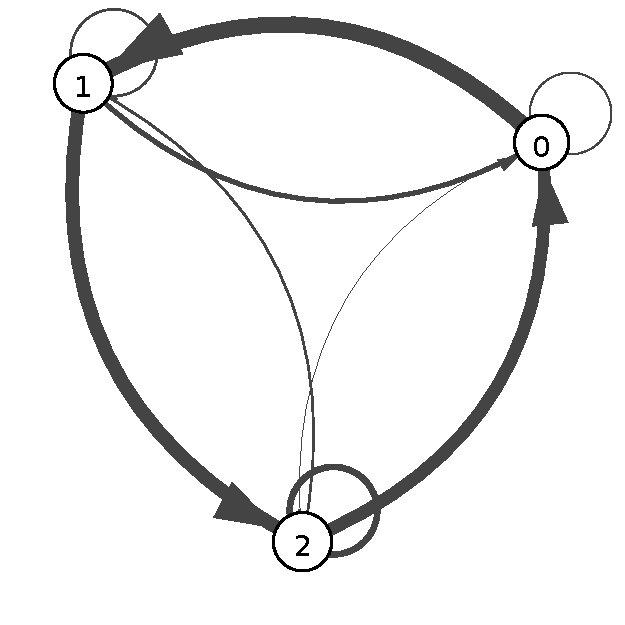
\includegraphics[width=150pt]{1215111126-model-3.pdf}
    \label{fig:first_sub}
}
\subfigure[The four highest emission probabilities for the states in of the HMM.]
{\small
\begin{tabular}[b]{| c | c | c |} \hline
    ~~State~~&~~Chord~~&Emission Probability \\\hline
    &$\mathrm{V^7}$&0.22 \\
    0&V&0.20 \\
    $D$&IV&0.12 \\
    &$\mathrm{vii^\circ}$&0.08 \\\hline
    &I&0.62 \\
    1&$\mathrm{vi^7}$&0.05 \\
    $T$&iii&0.04 \\
    &vi&0.03 \\\hline
    &V&0.20 \\
    2&IV&0.12 \\
    $P$&Vsus4&0.07 \\
    &$\mathrm{ii^7}$&0.07 \\\hline
   \end{tabular}
}
    \caption{Characteristic HMM corresponding to the maximum silhouette width in Fig. 1a., with $k=3$. Compare with Example 6 in White.}
    \label{fig:sample_figure_2}
\vspace{-10pt}
\end{figure}

\begin{figure}
\vspace{-25pt}
    \centering
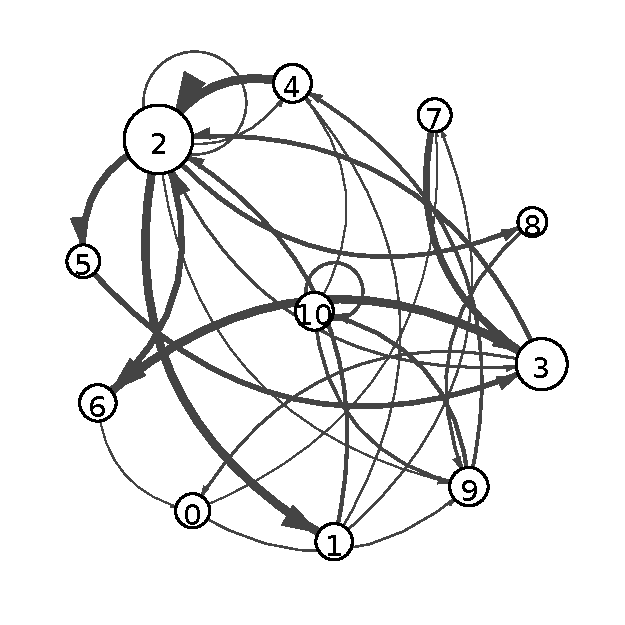
\includegraphics[width=200pt]{1215111126-model-11.pdf}
    \label{fig:first_sub}
    \caption{Characteristic HMM corresponding to a local maximum silhouette width in Fig. 1b., with $k=11$. Compare with Example 7 in White.}
    \label{fig:sample_figure_3}
\vspace{-10pt}
\end{figure}

\section{Discussion}
Overall, our results verify that HMMs trained on a collection of musical works produce chord functions and transition probabilities that accurately describe the musical grammar. The descriptive power of this grammar is limited by the inherent limitations of HMMs (as compared to more powerful generative grammars). Our low silhouette scores suggest at least one crucial difference from White's experiment. A more precise detailing of White's methods (hopefully forthcoming) is necessary to pinpoint any differences. Given our lack of consistent silhouette scores for models with $k >3$, the difference is likely to be in the HMM training and decoding step.

Despite these differences, our methods produce results for a three-state solution that are nearly identical to White's, and our high-scoring models with more than three states bear similarities to White's 13-state model. We can verify that a fundamental grammar of tonic, pre-dominant, dominant cycles underpins Bach's chorales. Further investigation is needed to see if this technique produces meaningful results for other collections of music. If it does, it is a computationally cheap way to access and understand the musical grammar of a body of work, requiring no expert knowledge. This technique may be useful as an aide to music theorists, or as a tool in genre classification based on shared musical grammars.

\section{ Acknowledgments}
I am lucky to be at the nexus of a few enthusiastic people who know a lot more than me. Thanks to Joti Rockwell for introducing me to the topic of Markov music analysis, Christopher White for his initial research and his advice, and America Chambers for teaching Bayesian networks and Markov models cogently.

\bibliography{ai}
\bibliographystyle{unsrtnat}
\end{document}
